\begin{frame}{Les Blockchain Bridges}
    \begin{figure}
        \centering
        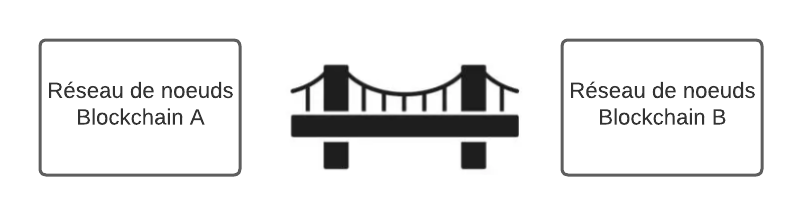
\includegraphics[scale = 1]{centralisation/img_bridges/Pont.png}
    \end{figure}
\end{frame}

\begin{frame}{Trusted Blockchain Bridge}
    Des informations clés: 
        \begin{itemize}
            \item Vérification de la transaction de manière externe.
            \item Dépendence avec l'opérateur du \textit{bridge}.
            \item Rapides.
            \item Rentables.
        \end{itemize}
    \end{frame}
    
    \begin{frame}{Trustless Blockchain Bridge}
    Des informations clés: 
    \begin{itemize}
        \item Dépend des chaînes sous-jacentes.
        \item Plus fiables que les \textit{Trusted Bridges}.
        \item Les utilisateurs contrôlent leurs actifs.
    \end{itemize}
    \end{frame}

\begin{frame}{Verrouiller et Frapper}
    \begin{figure}
        \centering
        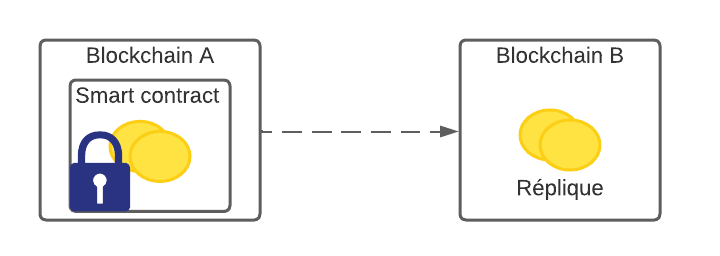
\includegraphics[scale = 1]{centralisation/img_bridges/LockAndMint.png}
    \end{figure}
\end{frame}

\begin{frame}{Détruire et Frapper}
    \begin{figure}
        \centering
        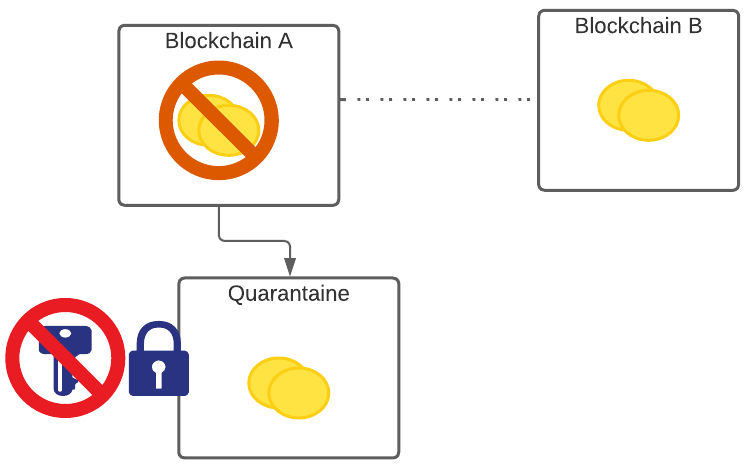
\includegraphics[scale = 0.7]{centralisation/img_bridges/BurnAndMint.png}
    \end{figure}
\end{frame}

\begin{frame}{Atomic Swaps}
    \begin{figure}
        \centering
        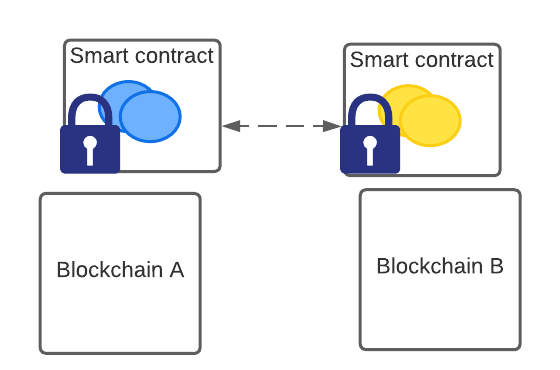
\includegraphics[scale = 1]{centralisation/img_bridges/AtomicSwap.png}
    \end{figure}
\end{frame}

\begin{frame}{Déroulement d'une transaction}
    \begin{figure}
        \centering
        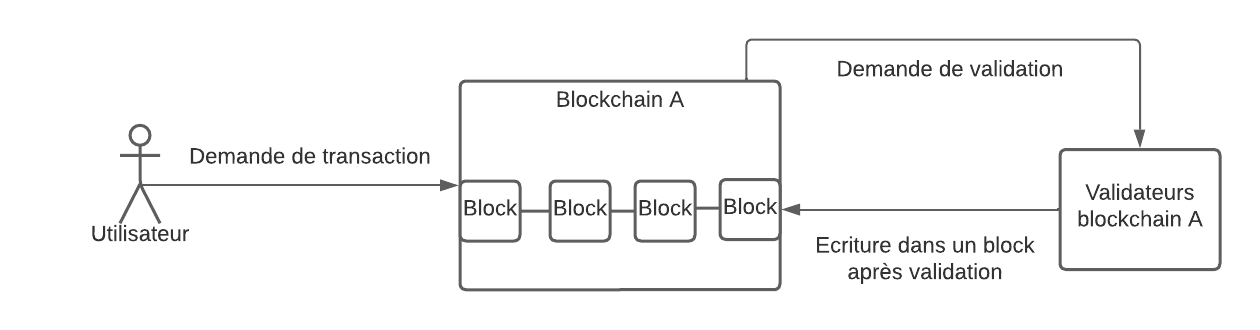
\includegraphics[scale = 0.6]{centralisation/img_bridges/Transaction1.png}
    \end{figure}
\end{frame}

\begin{frame}{Déroulement d'une transaction}
    \begin{figure}
        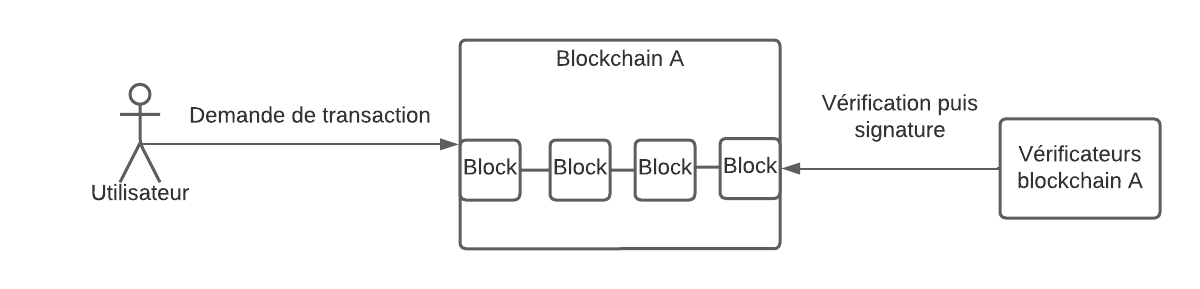
\includegraphics[scale = 0.65]{centralisation/img_bridges/Transaction2.png}
    \end{figure}
\end{frame}

\begin{frame}{Déroulement d'une transaction}
    \begin{figure}
        \centering
        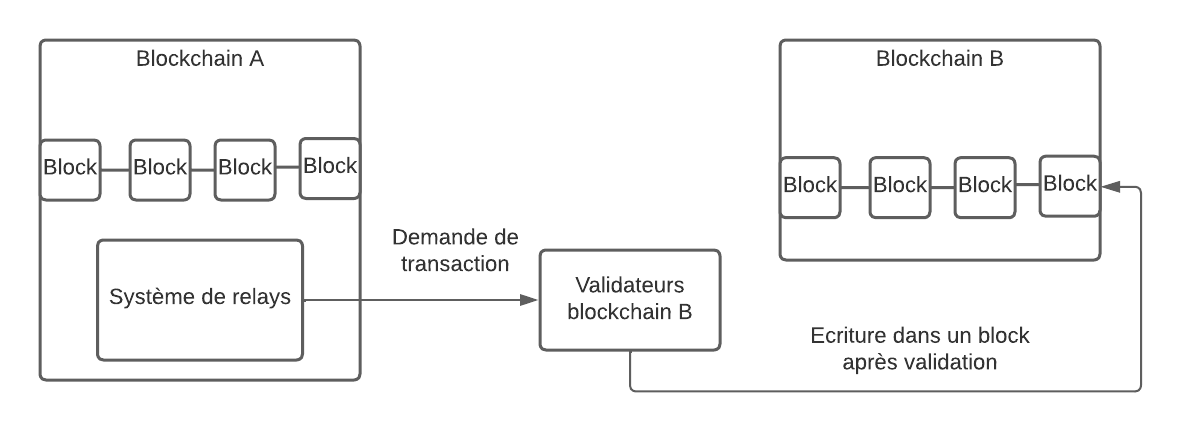
\includegraphics[scale = 0.65]{centralisation/img_bridges/Transaction3.png}
    \end{figure}
\end{frame}

\begin{frame}{Vérification locale, native et externe}
    \begin{figure}
        \centering
        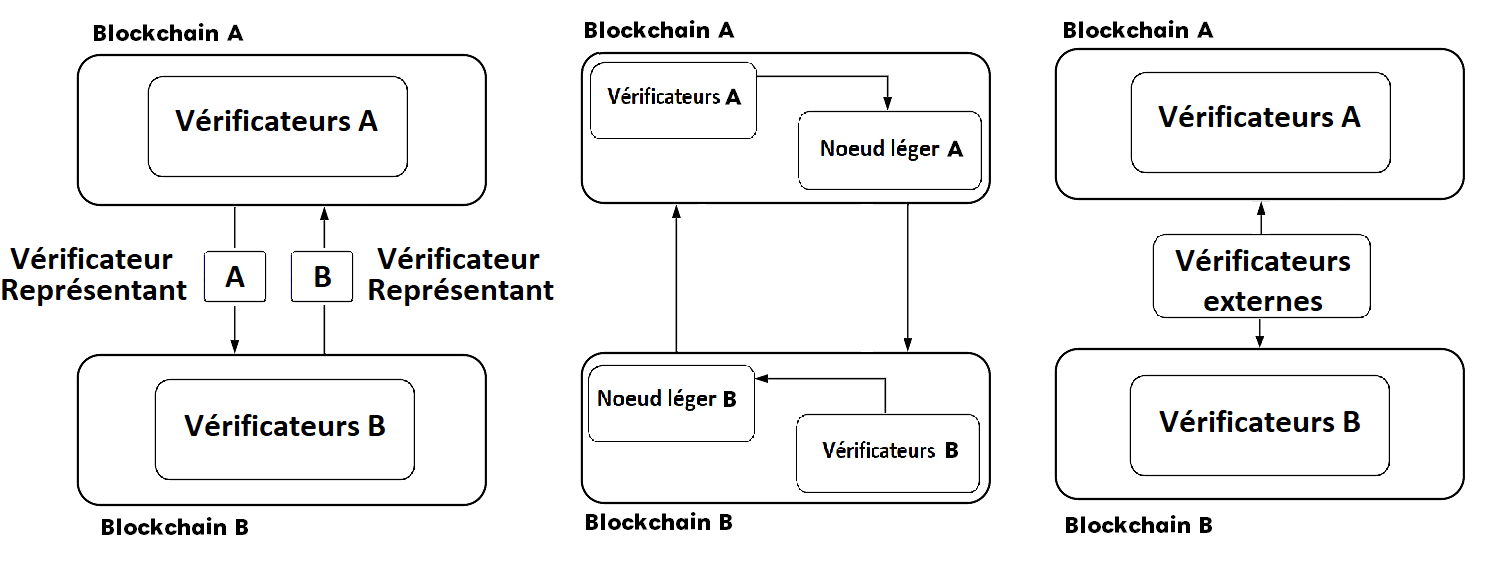
\includegraphics[scale = 0.4]{centralisation/img_bridges/DiagrammeResumeVerif.png}
    \end{figure}
\end{frame}

    
\begin{frame}{Les faiblesses des bridges}
    \begin{itemize}
        \item \textit{Trustless Bridges} : Les \textit{smart contracts} et l'erreur humaine.
        \item \textit{Trusted Bridges} : Les fraudes \textit{rug pull}.
        \item Une technologie récente.
    \end{itemize}
    \end{frame}

\begin{frame}{Le trilemme de l’interopérabilité}
    Repose sur 3 notions: 
    \begin{figure}
        \centering
        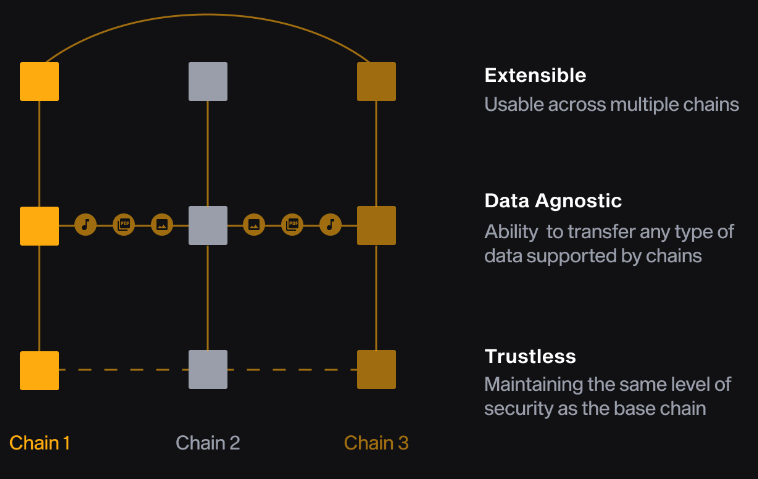
\includegraphics[scale = 0.7]{centralisation/img_bridges/3notions.png}
    \end{figure}
    \end{frame}

\begin{frame}{Solution optimiste}
    \begin{figure}
       \centering
       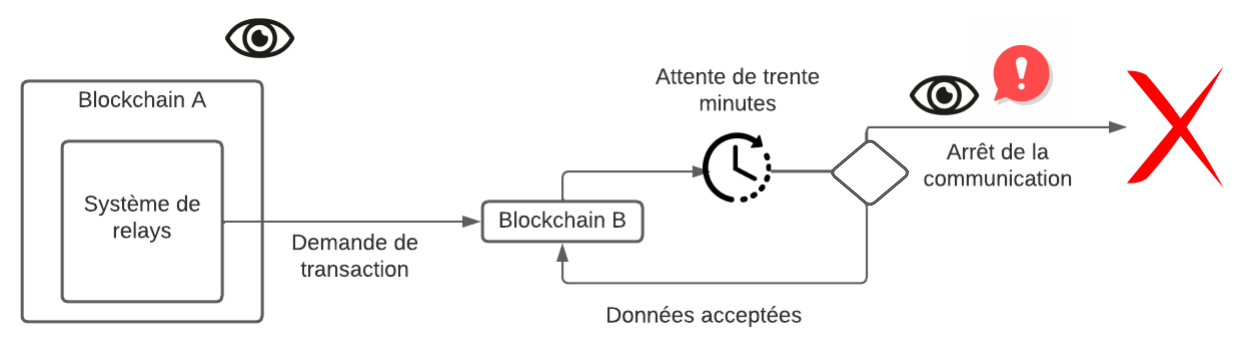
\includegraphics[scale = 0.6]{centralisation/img_bridges/VerifOptimiste.png}
    \end{figure}
\end{frame}    

\begin{frame}{Possibles faiblesses et leurs solutions}
\begin{itemize}
    \item \textit{Updater DoS}
        \begin{itemize}
            \item Mécanisme de substitution.
            \item Sanction financière et exclusion.
        \end{itemize}
    \item \textit{Updater Fraud} \begin{itemize} \item Sanction financière et exclusion. \end{itemize}
    \item \textit{Watcher DoS} 
        \begin{itemize}
            \item Vérificateurs approuvés.
            \item Signalement de fraude payant.
            \item Sanction financière et exclusion.
        \end{itemize}
\end{itemize}
\end{frame}
